\documentclass[11pt]{article}
\usepackage[margin=1 in, letterpaper]{geometry}
\usepackage{fontspec, graphicx, amsmath, amssymb, amsthm, array, physics, enumitem, cancel, multicol, float, dsfont}
\usepackage{latexsym, marvosym}
\usepackage[dvipsnames]{xcolor}

\setmainfont{Linux Libertine O}
\setsansfont{Linux Biolinum O}
\setmonofont{Latin Modern Mono}
\setmathrm{Latin Modern Math}
\theoremstyle{definition}
\newtheorem{theo}{\color{Maroon} Theorem}[section] 
\newtheorem{defin}[theo]{\color{Maroon} Definition}
\newtheorem{example}[theo]{\color{Maroon} Example}
\newtheorem{prob}[theo]{\color{Maroon} Problem}
% \newtheorem{example}[section]{\color{Maroon} Example}

\theoremstyle{remark}
\newtheorem*{soln}{\color{Maroon} Solution}

\newcommand{\R}{\mathbb{R}}
\newcommand{\Q}{\mathbb{Q}}
\newcommand{\Z}{\mathbb{Z}}
\newcommand{\N}{\mathbb{N}}
\newcommand{\Bin}{\text{Bin}}
\newcommand{\Bern}{\text{Bern}}

%%%%%%%%%%%%%%%%%%% Statistics %%%%%%%%%%%%%%%%%%%%
\newcommand{\E}[1]{\mathbb{E}\left[ #1 \right]}
\newcommand{\Prob}[1]{\mathbb{P}\left[ #1 \right]}
\newcommand{\cov}[2]{\textnormal{Cov}\left[ #1, #2 \right]}
\renewcommand{\var}[1]{\textnormal{Var}\left[ #1 \right]}
\newcommand{\Unif}{\textnormal{Unif}}
\newcommand{\Norm}{\mathcal{N}}
\newcommand{\ind}[1]{\mathds{1}_{#1}} 
\newcommand{\NBin}{\textnormal{NBin}}
\newcommand{\Geom}{\textnormal{Geom}}
\newcommand{\FS}{\textnormal{FS}}
\newcommand{\HGeom}{\textnormal{HGeom}}
\newcommand{\Pois}{\textnormal{Pois}}
\newcommand{\Expo}{\textnormal{Expo}}
\newcommand{\Beta}{\textnormal{Beta}}
\newcommand{\Gam}{\textnormal{Gamma}}

%%%%%%%%%%%%%%%%%%%%%%%%%%%%%%%%%%%%%%%%%%%%%%%%%%%%%%%%%%%%%%%%%%%%
\newcommand{\inserttitle}{Section 04}
\newcommand{\insertauthor}{Max Guo \& Seung Hwan An}
\newcommand{\insertcourse}{STAT 110}
%%%%%%%%%%%%%%%%%%%%%%%%%%%%%%%%%%%%%%%%%%%%%%%%%%%%%%%%%%%%%%%%%%%%

\usepackage{fancyhdr}
\setlength{\headheight}{15pt}
\pagestyle{fancy}
\fancyhf{}
\fancyhead[C]{\thepage}
\fancyhead[L]{\inserttitle}
\fancyhead[R]{\insertauthor}

%%%%%%%%%%%%%%%%%%%%%%%%%%%%%%%%%%%%%%%%%%%%%%%%%%%%%%%%%%%%%%%%%%%%

\begin{document}

{\noindent\Huge\bf  \\[0.1\baselineskip] {\inserttitle }}\\[2\baselineskip]
{{\bf \insertcourse}\\ {\textit{October 4, 2021}}} \hfill {\large \textsc{\insertauthor}}
\smallskip

\hfill \noindent \textit{Credits to Vincent Li and Dylan Li}

\section{Review}
\begin{description}

\item[Distribution $\neq$ Random Variable] A distribution is like a blueprint for a house, and the random variable is the house itself. Distributions can be described in a variety of ways, including the CDF or the PMF. The \textbf{support} of a random variable is the set of possible values that it can take.

\item[Probability Mass Function (PMF)] (Discrete Only) is a function that takes in the value $x$, and gives the probability that a random variable takes on the value $x$. The PMF is a positive-valued function over the support of $X$, and it is \textbf{required} to have $\sum_xP(X=x) = 1$ (normalization requirement).
\begin{center}
$P_X(x) = P(X=x)$
\end{center}

\item[Cumulative Distribution Function (CDF)] is a function that takes in the value $x$, and gives the probability that a random variable takes on the value at most $x$.
\[F(x) = P(X \leq x)\]

Why is it equivalent to specify a PMF versus a CDF?

\bigskip

\end{description}

\section{Expected Value, Linearity, and Symmetry}
\begin{description}
\item[Expected Value] (aka \emph{mean}, \emph{expectation}, or \emph{average}) can be thought of as the ``weighted average" of the possible outcomes of our random variable. Mathematically, if $x_1, x_2, x_3, \dots$ are all of the possible values that $X$ can take, the expected value of $X$ can be calculated as follows:
\begin{center}
$\E{X} = \sum\limits_{x} x P(X=x)$
\end{center}
Note that for \emph{any} $X$ and $Y$, $a$ and $b$ scaling coefficients and $c$ is our constant, the following property of \textbf{Linearity of Expectation} holds:

\[ \E{aX + bY + c} = a\E{X} + b\E{Y} + c \]

\Biohazard This, in general for a non-linear function is not true. That is: $$\E{g(X)} \neq g(\E{X})$$ e.g. $\E{X^2} \neq \E{X}^2$. We will in subsequent classes learn how to calculate these.

\Biohazard Note importantly that we have \textit{not} specified that $X$ and $Y$ need to be independent. Linearity of expectation holds for any $X,Y$.

\Biohazard An expectation is a property of a \textbf{distribution}. Hence, if two random variables have the same distribution, regardless of whether they are dependent or independent, they have the same expectation.

\item[Conditional Expected Value] is calculated like expectation, only conditioned on any event A. \begin{center}
$\E{X | A} = \sum\limits_{x}xP(X=x | A)$
\end{center}

\end{description}

\section{Indicator Random Variables}
\begin{description}
\item[Indicator Random Variables] is random variable that takes on either 1 or 0. The indicator is always an indicator of some event. If the event occurs, the indicator is 1, otherwise it is 0. They are useful for many problems that involve counting and expected value. 
\item[Distribution] $\ind{A} \sim \Bern(p)$ where $p = P(A)$
\item[Fundamental Bridge] The expectation of an indicator for $A$ is the probability of the event. $\E{I_A} = P(A)$. Notation: $$\ind{A} =
 \begin{cases}
   1 & A \text{ occurs} \\
   0 & A \text{ does not occur}
  \end{cases}$$

\begin{example}
Putnam Problem: if we have a permutation of $1, \ldots, n$, what is the expected number of local maxima (number that is greater than its neighbors?

Let $A_i$ be the event that $i$th number is a local maxima. Let us denote r.v. representing the number of local maxima to be $X$. Then, \begin{align*} \E{X} & = \E{ \sum_{i=1}^n \ind{A_i} } = \sum_{i=1}^n \E{\ind{A_i} } & \text{by Linearity of Expectation} \\ & = \sum_{i=1}^n P(A_i) & \text{by Fundamental Bridge} \\ & = 2 P(A_1) + (n-2) P(A_2) & \text{by Symmetry} \\ & = 2 \cdot \frac{1}{2} + (n-2) \cdot \frac{1}{3} = \frac{n+1}{3} \end{align*}
\end{example}

\end{description}

\section{Discrete Distributions}

\begin{description}
\item[Bernoulli] The Bernoulli distribution is the simplest case of the Binomial distribution, where we only have one trial, or $n=1$. $X$ is distributed \Bern($p$). Then:
\begin{description}
	\item[Story] $X$ ``succeeds" (is 1) with probability $p$, and $X$ ``fails" (is 0) with probability $1-p$.
	\item[Support] $\{0,1\}$.
	\item[Example] A fair coin flip is distributed \Bern($\frac{1}{2}$).
	\item[PMF] The probability mass function of a Bernoulli is:
\[P(X = x) = p^x(1-p)^{1-x}\]
or simply
\[P(X = x) = \begin{cases} p, & x = 1 \\ 1-p, & x = 0 \end{cases}\]
    \item[Expectation]
    $$ \E{X} = 0 \cdot P(X = 0) + 1 \cdot P(X=1) = p$$
\end{description}

\item[Binomial] $X$ is distributed \Bin($n,p$). Then:
\begin{description}
	\item[Story] $X$ is the number of ``successes" that we will achieve in $n$ independent trials, where each trial can be either a success or a failure, each with the same probability $p$ of success. We can also say that $X$ is a sum of multiple independent $Bern(p)$ random variables. Let $X \sim \Bin(n, p)$ and $X_j \sim \Bern(p)$, where all of the Bernoullis are independent. We can express the following:
	\[X = X_1 + X_2 + X_3 + \dots + X_n\]
	\item[Support] $\{0,1,\ldots,n\}$
	\item[Example] If Jeremy Lin makes 10 free throws and each one independently has a $\frac{3}{4}$ chance of getting in, then the number of free throws he makes is distributed  \Bin($10,\frac{3}{4}$), or, letting X be the number of free throws that he makes, X is a Binomial Random Variable distributed  \Bin($10,\frac{3}{4}$).
	\item[PMF] The probability mass function of a Binomial is:
    $$P(X = x) = \binom{n}{x} p^x(1-p)^{n-x}$$
    \item[Expectation] By linearity of expectation, this is $np$.
\end{description}

\item[Geometric] $X$ is distributed $\Geom(p)$. Then:
\begin{description}
	\item[Story] $X$ is the number of ``failures" that we will achieve before we achieve our first success. Our successes have probability $p$.
	\item[Support] $\{0,1,2, \ldots\}$
	\item[Example] Let $X$ be the number of tails I will flip before heads, then $X \sim \Geom(1/2)$
	\item[PMF] With $q = 1-p$, the probability mass function of a Geometric is:
        $$P(X = k) = q^kp$$
    \item[Expectation] This is a good opportunity to start practicing with summations. \begin{align*}
        \E{X} & = \sum_{k=0}^{\infty} k \cdot q^k p = p q \cdot \sum_{k=0}^{\infty} k \cdot q^{k-1} \\
        & = p q \cdot \sum_{k=0}^{\infty} \dv{}{q} \left( q^k \right) = p q \cdot \dv{}{q} \left( \sum_{k=0}^{\infty} q^k \right) \\
        & = p q \cdot \dv{}{q} \left( (1-q)^{-1} \right) = pq \cdot p^{-2} = q/p \\
    \end{align*}
\end{description}

\Biohazard We also talk about ``First Success'' distribution. This is the the total number of trails until our first success occurs. That is, if $Y=X+1$ and $X \sim \Geom(p)$, then $Y \sim \FS(p)$. Its support is $\{1,2,3,\ldots,\}$ and its PMF $$P(Y = k) = P(X+1 = k) = P(X = k-1) = q^{k-1}p$$ What is the expectation of $\FS(p)$ distributed r.v.? 

\pagebreak

\item[Negative Binomial] $X$ is distributed $\NBin(r, p)$. Then:
\begin{description}
	\item[Story] $X$ is the number of ``failures" that we will achieve before we achieve our $r$th success. Our successes have probability $p$. Note that with this story, if $X_i$ are iid $\Geom(p)$ distributed r.v.s, then $$ X = X_1 + X_2 + \ldots + X_r $$
	\item[Support] $\{0,1,2,\ldots\}$
	\item[Example] Let $X$ be the number of tails I will flip before 10 heads, then $X \sim \NBin(10,1/2)$
	\item[PMF] With $q = 1-p$, the probability mass function of a Negative Binomial is:
        $$P(X = n) = \binom{n+r - 1}{r -1}p^rq^n$$
    \item[Expectation] By linearity of expectation, it is $rq/p$. 
\end{description}

\item[Hypergeometric] $X$ is distributed $\HGeom(w, b, n)$. Then:
\begin{description}
	\item[Story] In a population of $b$ undesired objects and $w$ desired objects, $X$ is the number of ``successes" we will have in a draw of $n$ objects, without replacement. Hence we are given requirement that $w,b \geq n$.
	\item[Support] $\{0,1,\ldots,n\}$.
	\item[Examples] 1) We have only $b$ Weedles (failure) and $w$ Pikachus (success) in Viridian Forest. We encounter $n$ of the Pokemon in the forest, and $X$ is the number of Pikachus in our encounters. 2) The number of aces that you draw in 5 cards (without replacement). 3) You have $w$ white balls and $b$ black balls, and you draw $b$ balls. $X$ is the number of white balls you will draw in your sample. 4) Elk Problem - You have $N$ elk, you capture $n$ of them, tag them, and release them. Then you recollect a new sample of size $m$. How many tagged elk are now in the new sample?
	\item[PMF] The probability mass function of a Hypergeometric is:
        \[P(X = k) = \frac{\binom{w}{k}\binom{b}{n-k}}{\binom{w + b}{n}}\]
    \item[Expectation] Refer back to the story of a hypergeometric. Let $A_i$ be the event that $i$th object that we pick, we draw a success. Then, $X = \sum_{i=1}^n \ind{A_i}$, so $$\E{X} = \sum_{i=1}^n P(A_i) = n \frac{w}{b+w}$$
\end{description}
\end{description}

\section{Distribution Table}
\begin{center}
\renewcommand{\arraystretch}{2}
\begin{tabular}{cccccc}
\textbf{Distribution} & \textbf{PDF and Support} & \textbf{Expected Value}  & \textbf{Equivalent To}\\
\hline
\shortstack{Bernoulli \\ \Bern($p$)} & \shortstack{$P(X=1) = p$ \\$ P(X=0) = q$} & $p$ & $\Bin(1, p)$ \\
\hline
\shortstack{Binomial \\ \Bin($n, p$)} & \shortstack{$P(X=k) = {n \choose k}p^k(1-p)^{n-k}$  \\ $k \in \{0, 1, 2, \dots n\}$}& $np$ & Sum of $n$ iid Bern($p$) \\
\hline
\shortstack{Geometric \\ \Geom($p$)} & \shortstack{$P(X=k) = q^kp$  \\ $k \in \{$0, 1, 2, \dots $\}$}& $\frac{q}{p}$ &  \NBin($1, p$)\\
\hline
\shortstack{Negative Binomial \\ \NBin($r, p$)} & \shortstack{$P(X=n) = {n+r - 1 \choose r -1}p^rq^n$ \\ $n \in \{$0, 1, 2, \dots $\}$} & $r\frac{q}{p}$ &  Sum of $r$ iid Geom($p$)\\
\hline
\shortstack{Hypergeometric \\ \HGeom($w, b, n$)} & \shortstack{$P(X=k) = \frac{{w \choose k}{b \choose n-k}}{{w + b \choose n}}$ \\ $k \in \{0, 1, 2, \ldots \}$} & $n\frac{w}{b+w}$ & \\
\end{tabular}
\end{center}

\section{Practice Problems}
\vskip .2 in

% \fbox{\parbox{0.9 \textwidth}{}}

\begin{prob} Let $X$ be the r.v. representing the maximum of $n$ dice rolls. Find its CDF, then its PMF, and expectation. (For expectation, there is going to be summation in your answer, but try to simplify as much as possible)

\medskip

\fbox{\parbox{0.9 \textwidth}{In this case, it is much easier to find the CDF of $X$. Event $X \leq 4$ means that I have \textit{not} rolled a 5 or 6. Hence, $$P(X \leq k) = \left(\frac{k}{6}\right)^n $$ for $k = 1,\ldots, 6$. Hence, $$P(X=k) = P(X \leq k) - P(X \leq k-1) = \left(\frac{k}{6}\right)^n - \left(\frac{k-1}{6}\right)^n $$ Note that for any discrete r.v. whose support is $\{1, 2, \ldots, n \}$ $$\E{X} = \sum_{i=1}^n i (F(i)-F(i-1)) = nF(n) - F(n-1) - F(n-2) \ldots - F(1) = n - \sum_{i=1}^{n-1} F(i) $$ (An analogous result for continuous distribution will come up later in the course). Thus, $$\E{X} = 6 - 6^{-n} \sum_{i=1}^5 i^n $$ Does this answer make sense? If $n=1$, then this is $3.5$, which is just the expectation of a dice roll. If $n$ is super large, then the second term converges to zero, so the answer converges to $6$ (which just says after enough dice rolls, your maximum roll is surely a six)}}

\end{prob}

\pagebreak

\begin{prob} Suppose you have a $n \times n$ grid. Each turn, you randomly pick a cell, and color the $3 \times 3$ grid around it. That is, the cell you picked, and all the adjacent (including diagonally adjacent cells) are colored. What is the expected number of colored cells after $k$ turns? (It is ok to leave the answer unsimplified)

\medskip

\fbox{\parbox{0.9 \textwidth}{Let us define event $A_i$ as the event that $i$th cell is colored at the end. Then, if $X$ is the total number of colored cells after $k$ turns, then $X = \sum_{i=1}^{n^2} \ind{A_i}$. Note that there are $(n-2)^2$ ``center'' cells, $4(n-2)$ ``edge'' cells, and $4$ ``corner'' cells. \begin{center}
    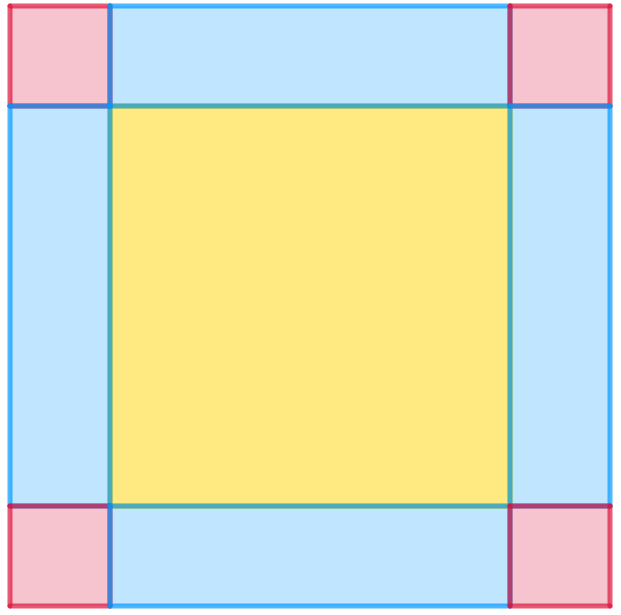
\includegraphics[width=0.3\textwidth]{image/grid.png}
\end{center}
For a center cell, if any of the 9 cells (itself, and 8 cells around it) is picked, then it will be colored. Hence the probability that it will be colored after $k$ rounds is $$1 - \left( 1 - \frac{9}{n^2} \right)^k$$ For an edge cell, for similar reasoning, the probability it will be colored after $k$ rounds is $$1 - \left( 1 - \frac{6}{n^2} \right)^k$$ and for a corner cell, $$1 - \left( 1 - \frac{4}{n^2} \right)^k$$ Therefore, \begin{align*}\E{X} & = \E{\sum_{i=1}^{n^2} \ind{A_i}} = (n-2)^2 \E{A_{\text{center}}} + 4(n-2) \E{A_{\text{edge}}} + 4 \E{A_{\text{corner}}} \\
& = (n-2)^2 \left( 1 - \left( 1 - \frac{9}{n^2} \right)^k \right) + 4(n-2) \left( 1 - \left( 1 - \frac{6}{n^2} \right)^k \right) + 4 \left( 1 - \left( 1 - \frac{4}{n^2} \right)^k \right) \\
& = n^2 - \left( (n-2)^2 \left( 1 - \frac{9}{n^2} \right)^k + 4(n-2) \left( 1 - \frac{6}{n^2} \right)^k + 4 \left( 1 - \frac{4}{n^2} \right)^k \right)
\end{align*}
Note that trying to get the distribution of $X$ is going to be extremely difficult. Expectation in general is much much easier to calculate than the general distribution due to its linearity.}}

\end{prob}

\pagebreak

\begin{prob} (Balls in Boxes, V2) 
Assume $m, n-m \geq k$ in all of these problems.
\begin{enumerate}[label=\alph*)]
    \item Suppose you have $n$ boxes, and $k$ balls. You randomly distribute $k$ balls into $n$ boxes (in particular here, you are allowed to have empty boxes). You then randomly pick $m$ boxes, and count the total number of balls in those boxes, and call this r.v. $X$. What is the expectation of $X$? 
    
    % \vspace{2 in}
    
    \fbox{\parbox{0.9 \textwidth}{
    For $i$th box, for $i \in [1:m]$, denote $X_i$ to be the number of balls in it. Hence $\E{X} = \sum_{i=1}^m \E{X_i}$. Now, denote the event that $j$th ball is put into box $i$ to be $A^{j}_i$ for $j \in [1:k]$. Hence $X_i = \sum_{j=1}^k \ind{A^j_i}$, so, $\E{X_i} = k P(A^j_i) = k/n$. Hence, the answer is $mk/n$.}}
    
    \item Now, suppose you are given an extra restriction that you are not allowed to have more than one ball in a box (i.e. you are essentially picking $k$ boxes out of $n$ boxes to put balls in). You again randomly pick $m$ boxes, and count the total number of balls in those boxes, and denote it to be $X'$. What is the distribution and expectation of $X'$?
    
    % \vspace{2 in}
    
    \fbox{\parbox{0.9 \textwidth}{
    Think from a ball's perspective. Whether you first distribute the balls and then pick the boxes, or pick the boxes and then distribute the balls is unimportant. So first pick $m$ boxes, so that $n-m$ boxes will be not chosen. Then out of $n$ total boxes, you draw $k$ of them. This is exactly the story of a hypergeometric, where you have $m$ desired boxes (ones you chose), and $n-m$ undesired boxes (ones you didn't chose), and you are drawing $k$ of them. So this is $\HGeom(m,n-m,k)$. The expectation is $km/n$. }}

    \item Now give the distribution of $X$.
    
    \fbox{\parbox{0.9 \textwidth}{
    Now use the same logic as part (b), first pick $m$ boxes and then distribute $k$ balls. Each ball can either be a part of $m$ boxes or not be a part of $m$ boxes, and this choice for each ball is independent of another. Hence this is $\Bin(k,m/n)$.}}

\end{enumerate}
\end{prob}

\end{document}